Pour accéder à l’interface d’administration du site, il suffit d’entrer l’adresse de celui-ci accompagné de "/admin". Exemple : \href{http://asmae.herokuapp.com/admin}{http://asmae.herokuapp.com/admin}\\
Vous êtes alors redirigé vers une page qui vous invite à entrer votre login et mot de passe (administrateur) telle que celle-ci :

\begin{figure}[H]
\centering
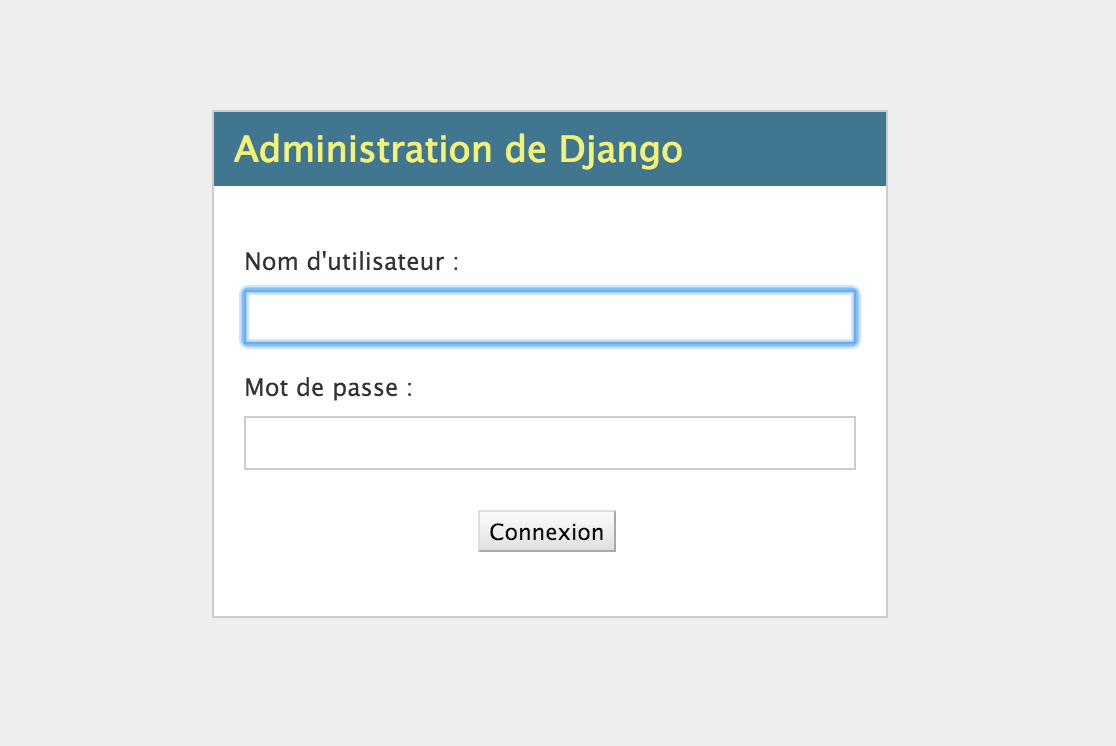
\includegraphics[scale=0.4]{connexion.png}
\caption{Connexion à l'interface administrateur}
\end{figure}

Une fois connecté, vous êtes redirigé vers la page d'accueil de l'interface administrateur qui se présente de la manière suivante :

\begin{figure}[H]
\centering
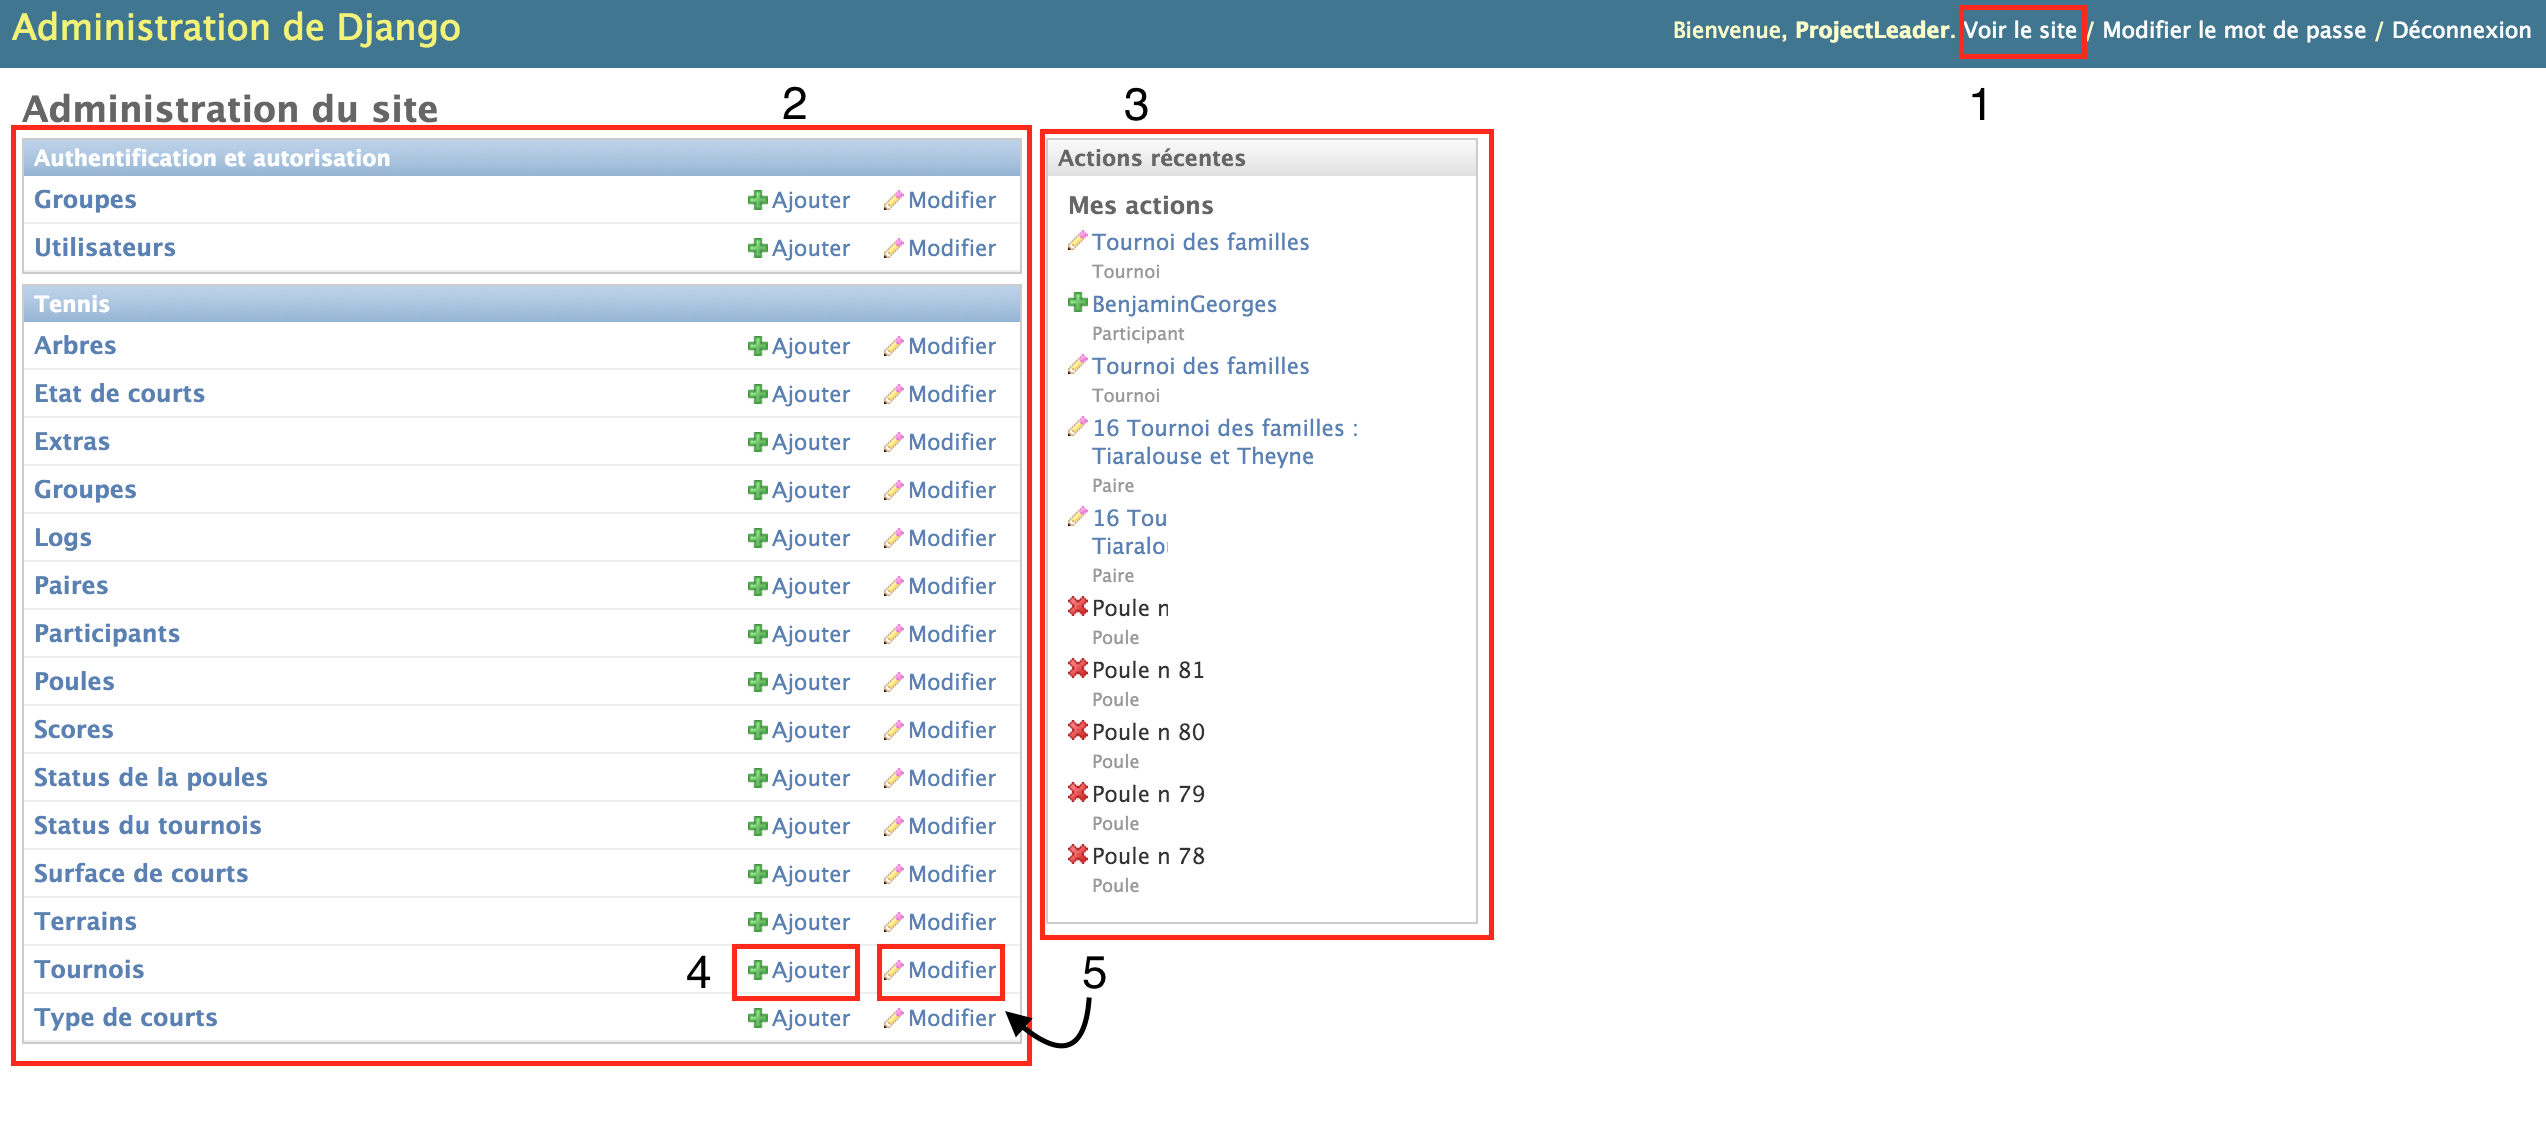
\includegraphics[scale=0.3]{accueil.png}
\caption{Accueil de l'interface administrateur}
\end{figure}

\begin{enumerate}
\item Lien direct pour accéder au site web
\item Liste des différentes tables présentes dans la base de données. Il est possible d’ajouter des entrées à ces tables, de les modifier ou de les supprimer. Il est par contre impossible d’ajouter de nouvelles tables via cette interface (pour ce faire voir page ... de ce document)
\item Liste des dix dernières actions effectuées par l’administrateur
\item Lien direct pour ajouter une entrée à la table correspondante. Ce lien nous redirige vers la fenêtre suivante :

\begin{figure}[H]
\centering
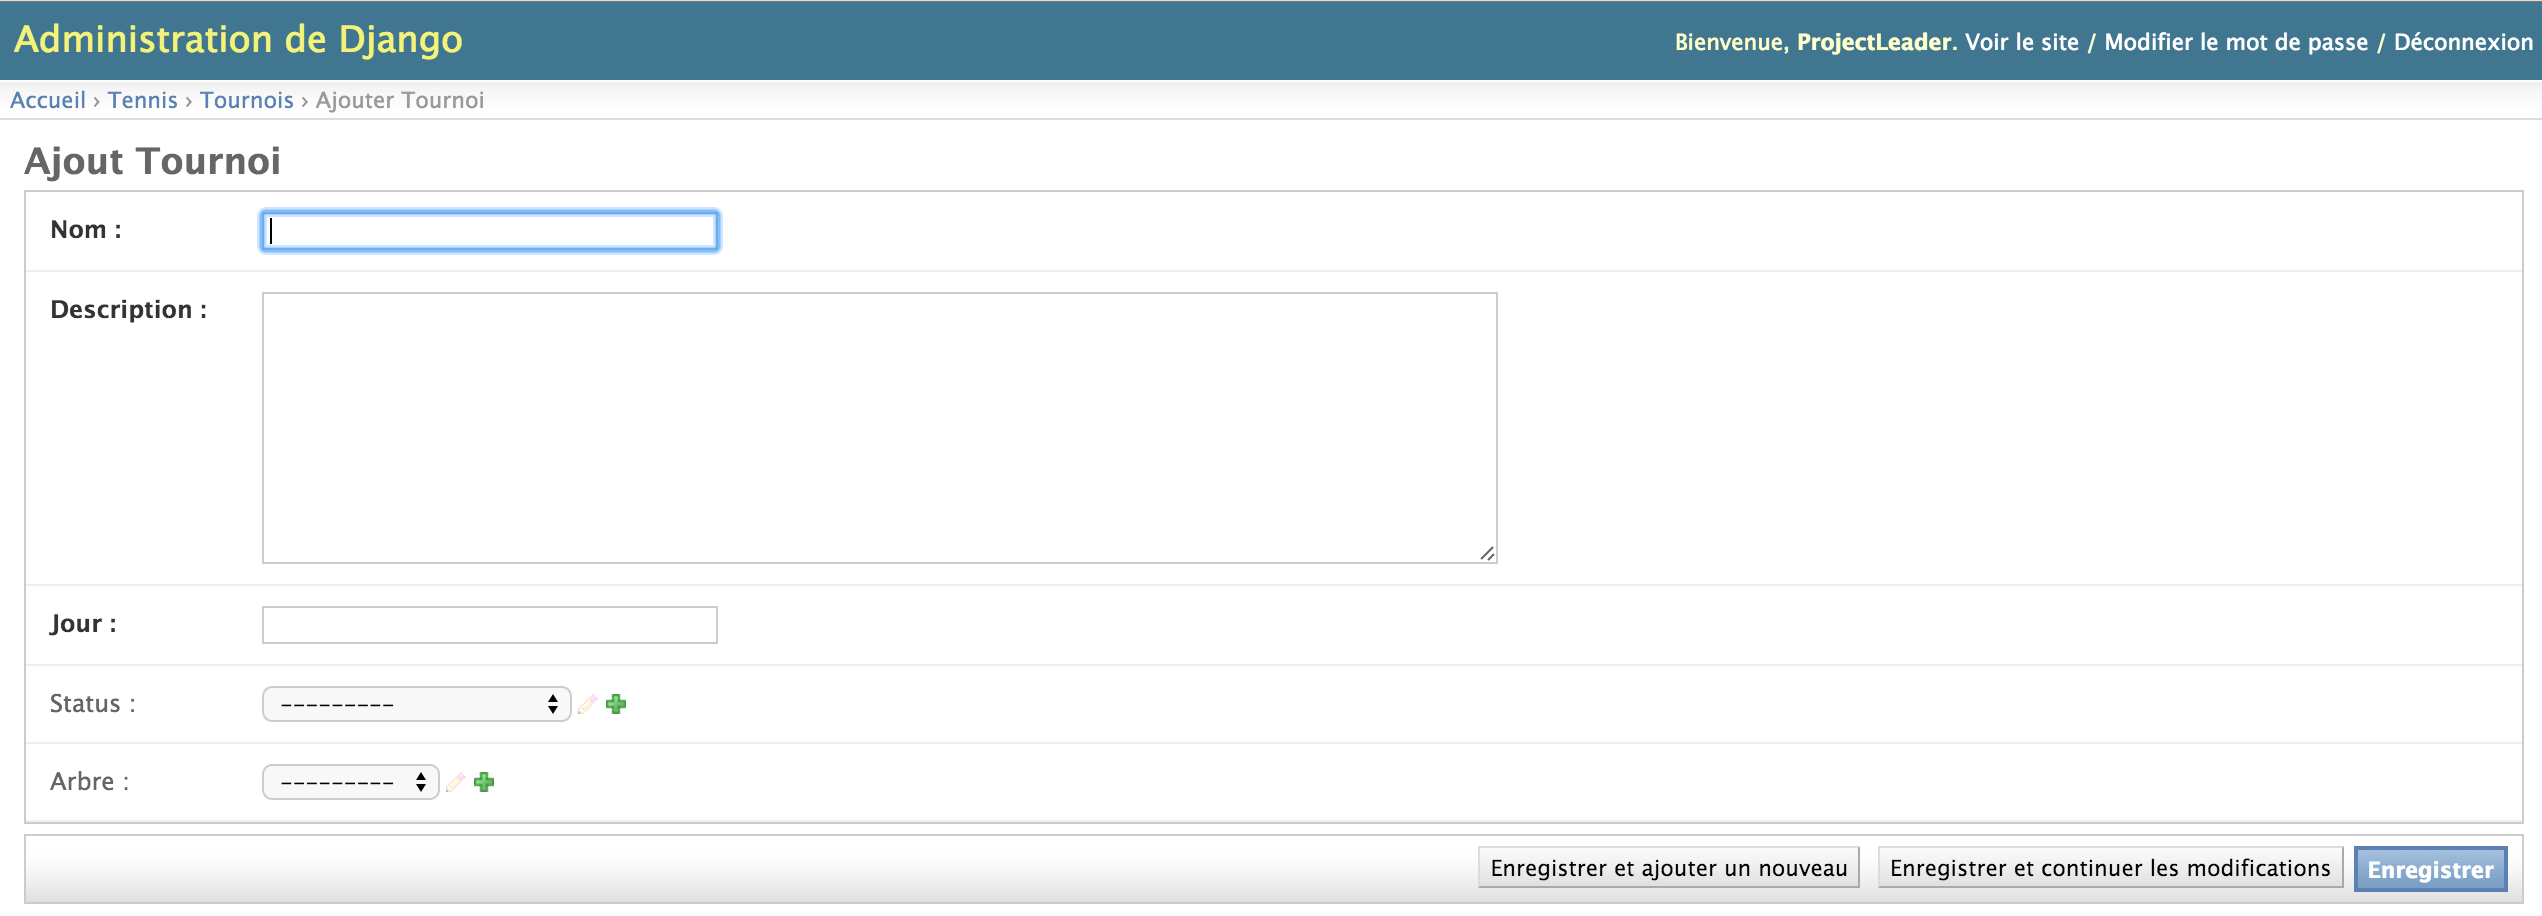
\includegraphics[scale=0.3]{add.png}
\caption{Ajouter une nouvelle entrée à la table "Tournoi"}
\end{figure}

Dans ce cas-ci, il est possible d'ajouter un nouveau tournoi en remplissant les différents champs et en appuyant ensuite sur le bouton "Enregistrer".

\item Lien direct pour modifier des entrées dans la table correspondante. Ce lien nous redirige vers la fenêtre suivante :

\begin{figure}[H]
\centering
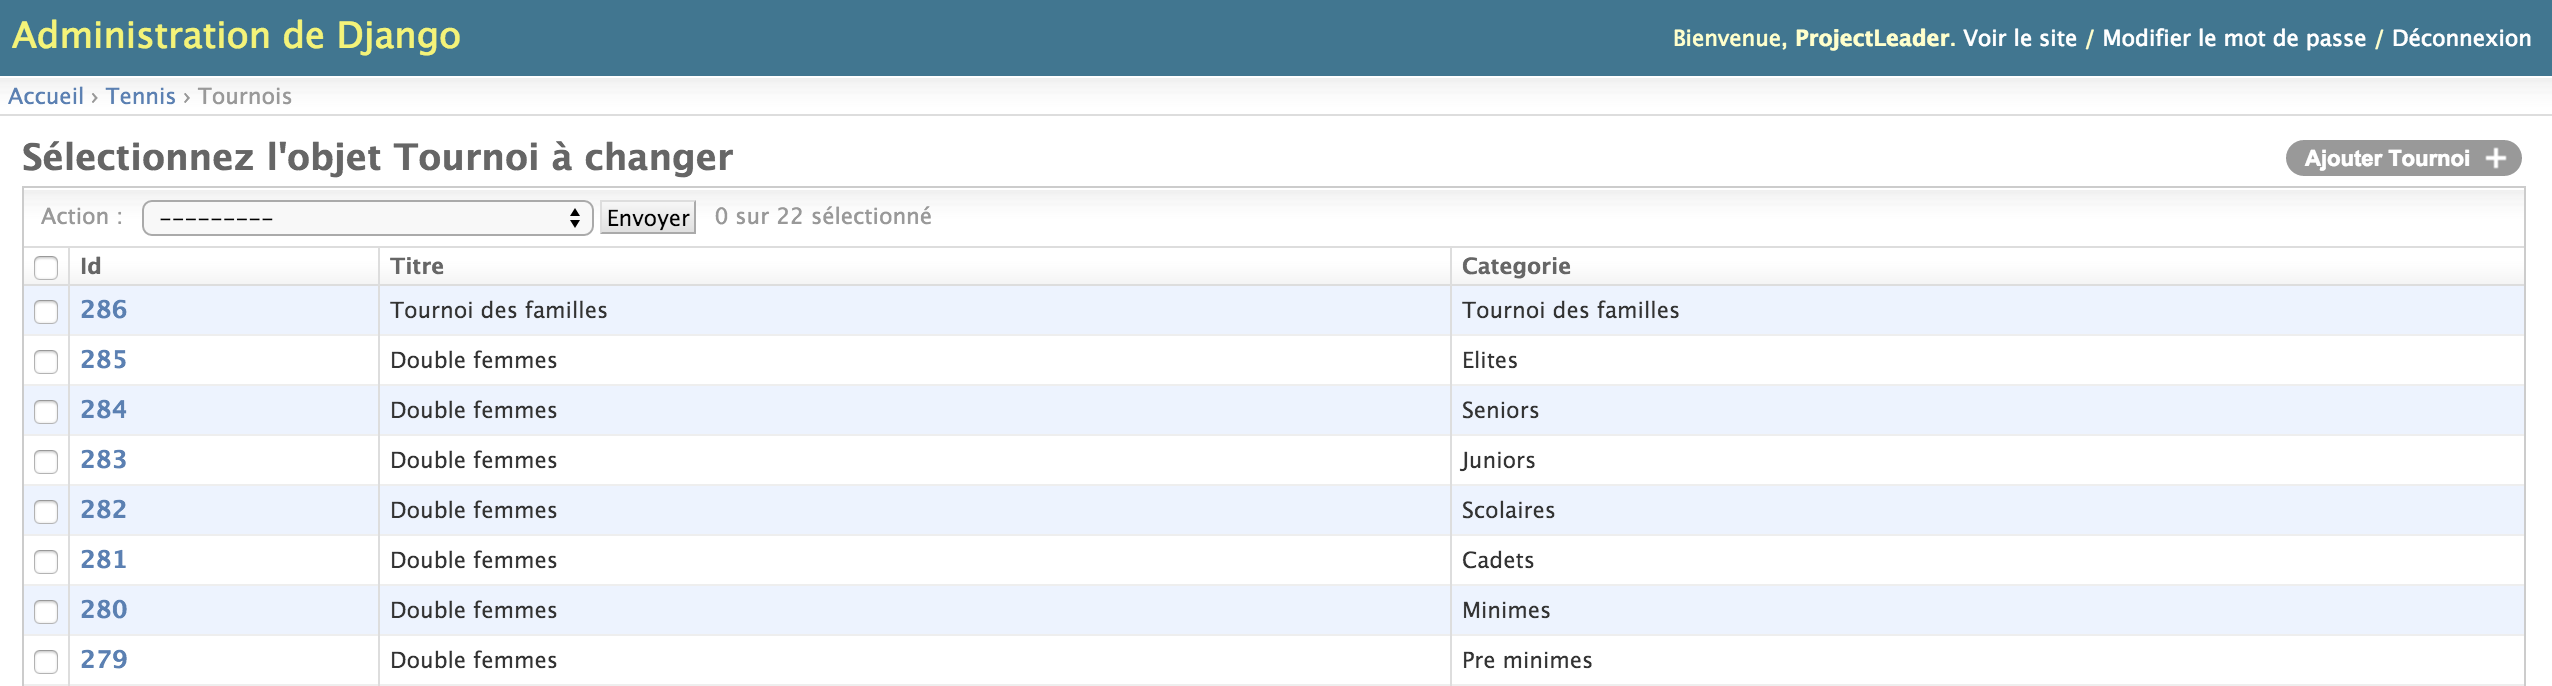
\includegraphics[scale=0.3]{entrees.png}
\caption{Entrées de la table "Tournoi"}
\end{figure}

Cette fenêtre reprend les différentes entrées de la table sélectionnée. Ces entrées peuvent être modifiées en cliquant sur le nom de celles-ci. On peut également à partir de cette fenêtre supprimer plusieurs entrées ou encore en ajouter.\\

Lorsque l’on clique sur le nom d’une entrée de la table, nous arrivons sur la fenêtre suivante :

\begin{figure}[H]
\centering
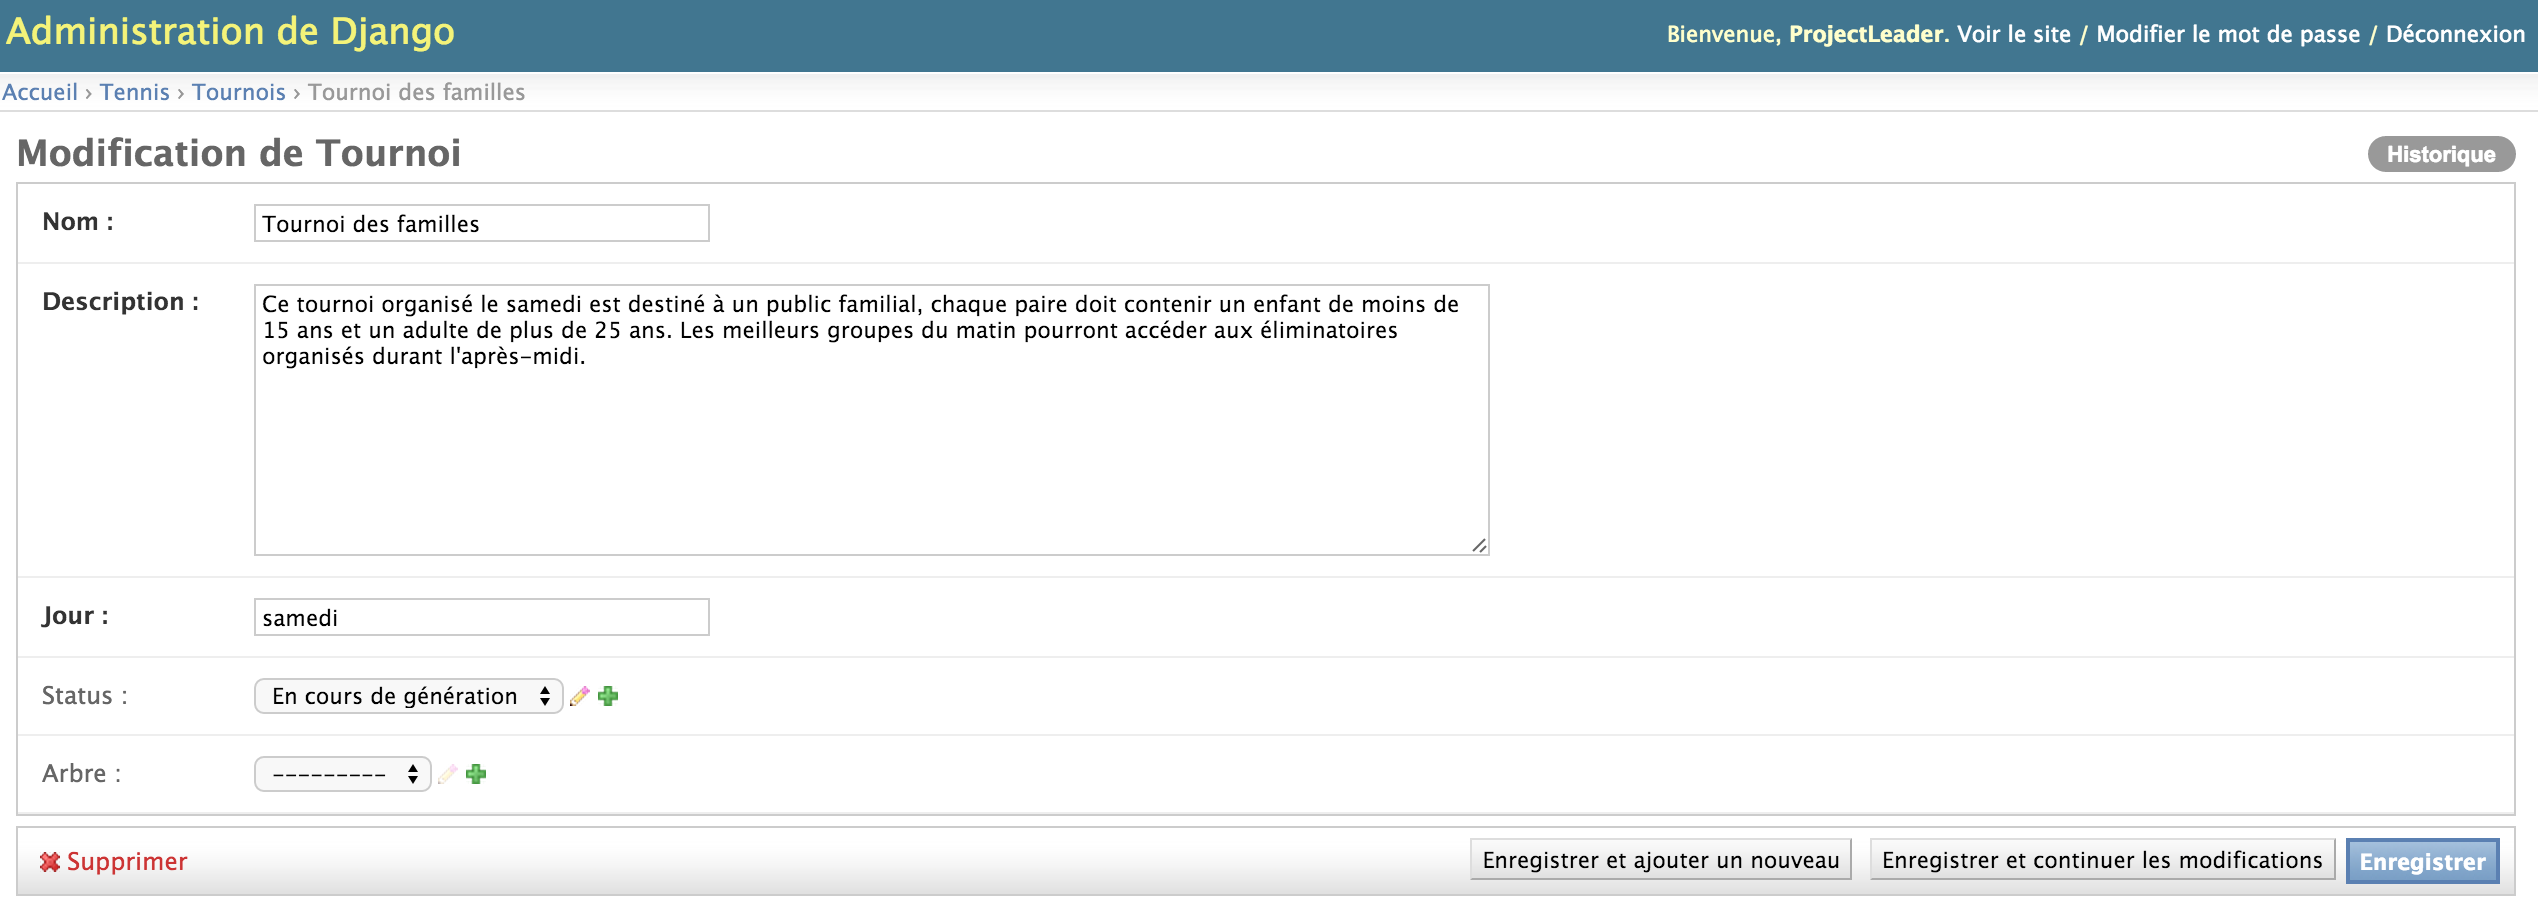
\includegraphics[scale=0.3]{edit.png}
\caption{Editer une entrée de la table "Tournoi"}
\end{figure}

Cette fenêtre reprend les différentes informations concernant l’entrée sélectionnée et nous permet de les éditer directement via les champs visibles sur la capture ci-dessus. On peut également observer l’historique des modifications de cette entrée en cliquant sur le bouton "Historique". Nous obtenons ainsi la fenêtre suivante :

\begin{figure}[H]
\centering
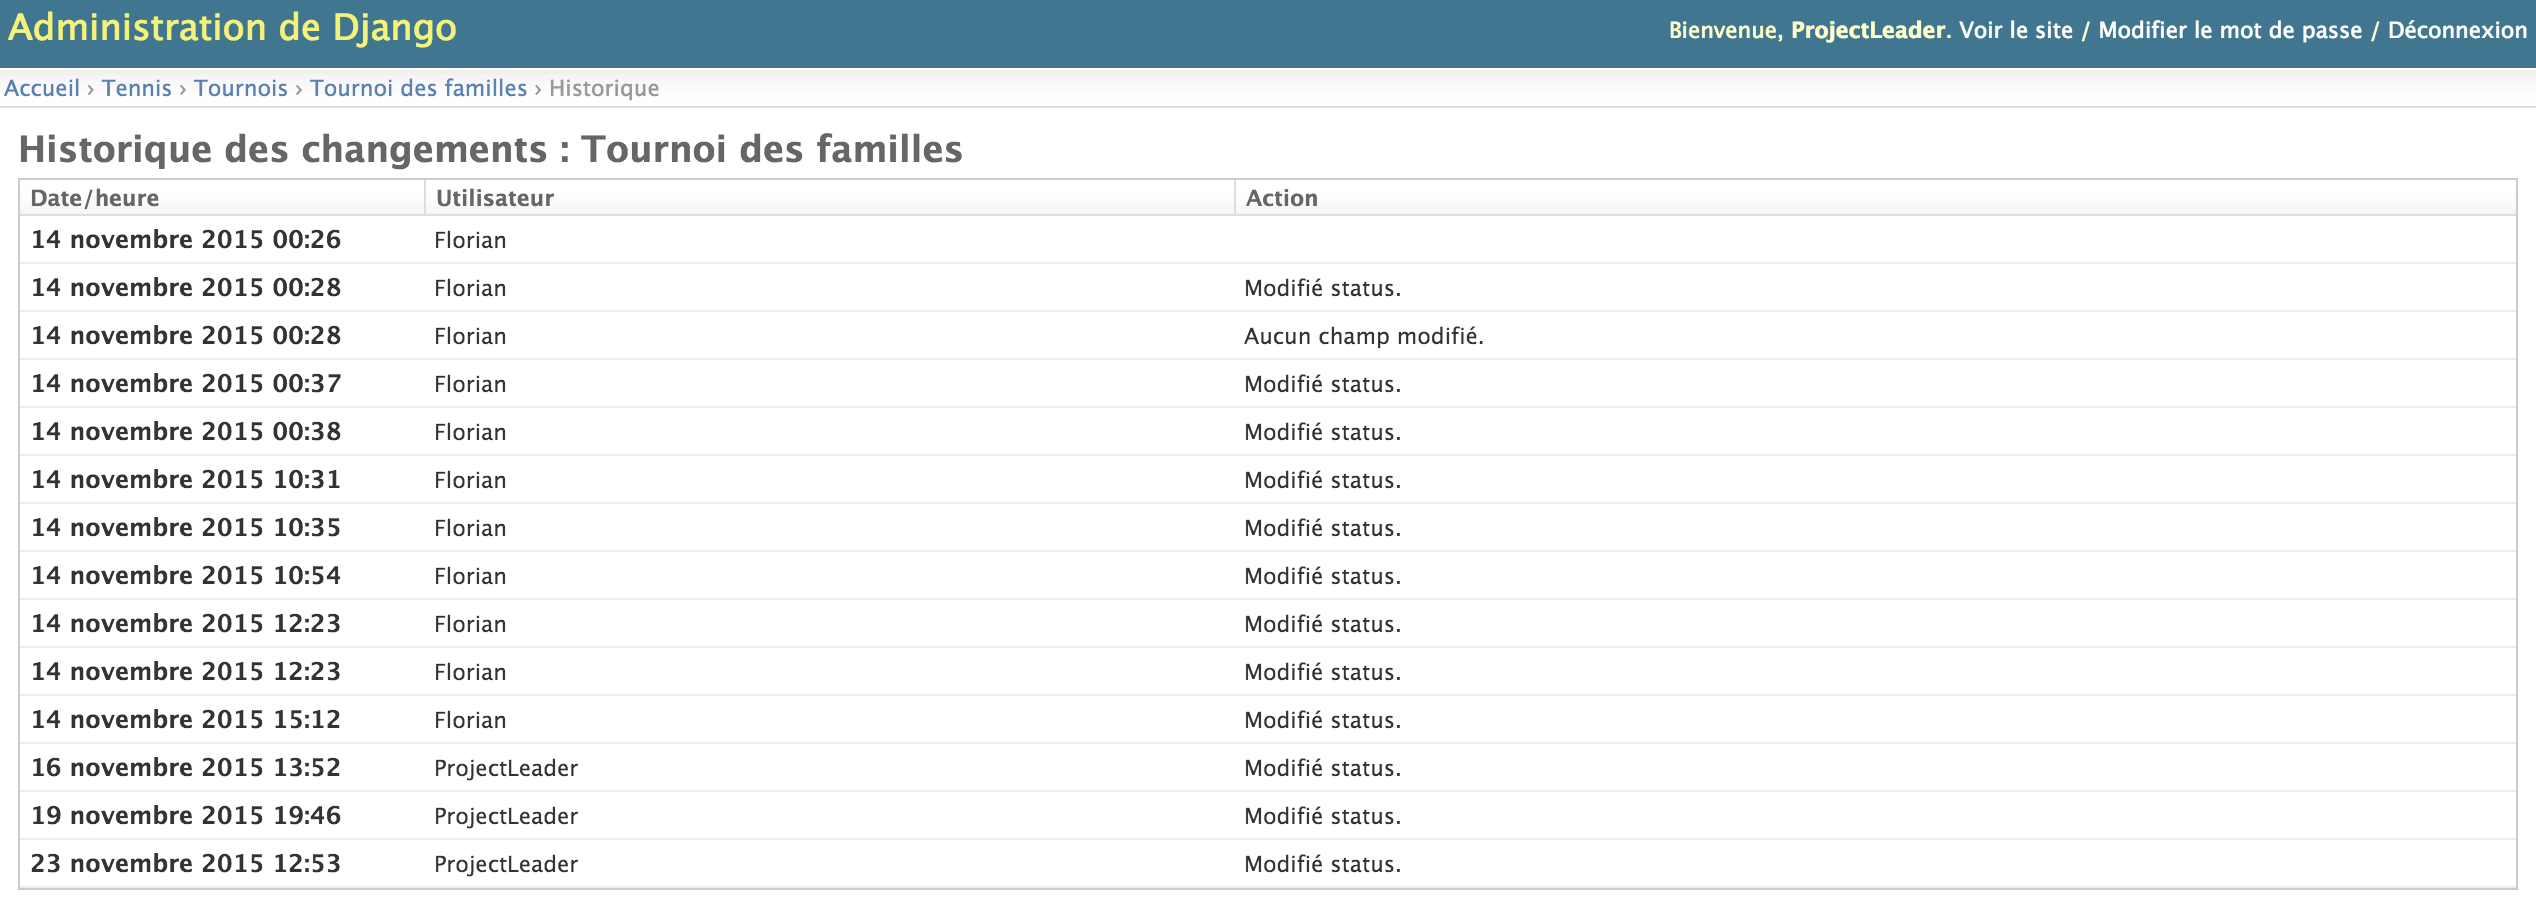
\includegraphics[scale=0.3]{historique.png}
\caption{Historique des modifications de l'entrée choisie}
\end{figure}
\end{enumerate}